%!TEX root = ../thesis.tex

\chapter[discussion]{Discussion}\label{chp:discussion}
% ~5 pages
%
% OUTLINE:
% - paper-hierarchical:
%   - Suitability of VAEs for representation learning (minimization of mutual information and sensitivity to implicit prior such as architecture)
% - paper-benchmarking
%   - Inferiority of probabilistic methods compared to self-supervised learning. 
% - 


\section{\Cref{chp:paper-hierarchical} revisited: \dots}

\lesstodo[inline]{Discuss sensitivity to ``implicit" prior such as architecture (and probably optimization method and other). Include reference to \parencite{huszar_is_2017} discussing the usefulness of using a maximum likelihood objective for representation learning in generative models.}
\lesstodo[inline]{Discuss whether VAEs are even suitable for representation learning due to them minimizing a mutual information term in the ELBO (derive this form).}
\lesstodo[inline]{Discuss some recent work e.g. \cref{morningstar_density_2021}}


\section{\Cref{chp:paper-benchmarking} revisited: Bested?}

\lesstodo[inline]{Discuss whether variational autoencoders are viable for learning good representations for speech for downstream tasks when alternatives such as SSL method exist.}
\lesstodo[inline]{Out-of-distribution detection on speech?}


\section{\Cref{chp:paper-review} revisited: \dots} \label{sec:discussion-paper-review}

\lesstodo[inline]{Are self-supervised speech representations useful for unsupervised uncertainty estimation? \parencite{nava_stateconsistency_2021, nava_uncertaintyaware_2021} Within robotics but not really related.}
% Since the main focus within self-supervised learning has been on improving downstream task performance, very limited work, if any, has investigated self-supervised representations in terms of uncertainty estimation. 
% However, in the context of medical applications where data can be abundant but labels are sparse, unsupervised uncertainty estimation is a very interesting direction for future work.
\lesstodo[inline]{OOD data: Generalization or detection (https://arxiv.org/pdf/2110.11334.pdf)?}


\section{\Cref{chp:paper-retrospective} revisited: Uncertainty}
The work in \textcite{wenstrup_retrospective_2023} focuses on predictive performance and an analysis of feature importance but does not explicitly consider uncertainty estimation. 




\begin{figure}
    \begin{subfigure}[c]{0.48\columnwidth}
        \centering
        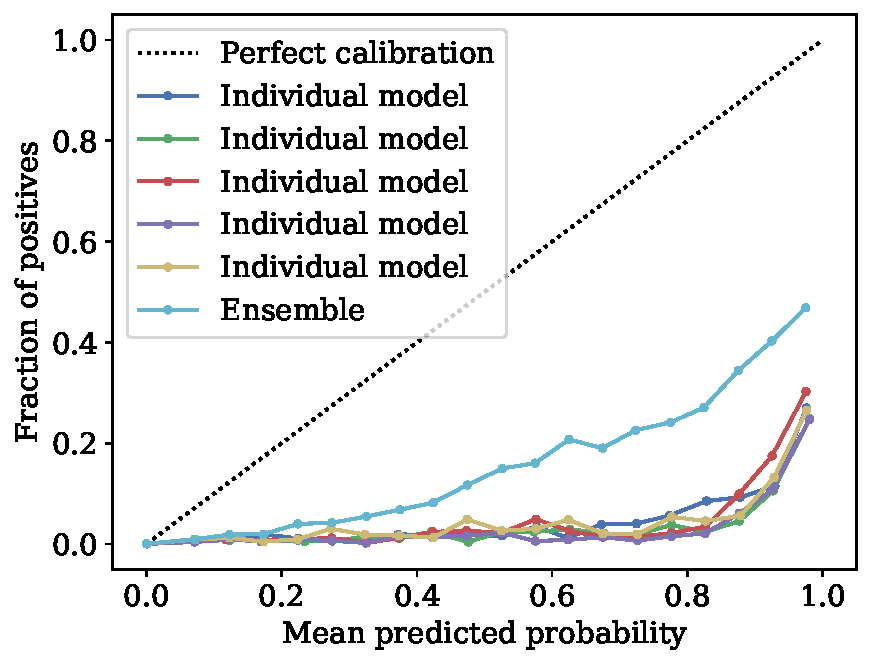
\includegraphics[width=1\columnwidth]{python_plotting/calibration_curve_ensemble_and_all_models_uncalibrated.pdf}
        % \caption{}
        % \label{fig_discussion:calibration_curve_ensemble_and_all_models_uncalibrated}
    \end{subfigure}
    % \hfill
    \begin{subfigure}[c]{0.48\columnwidth}
        \centering
        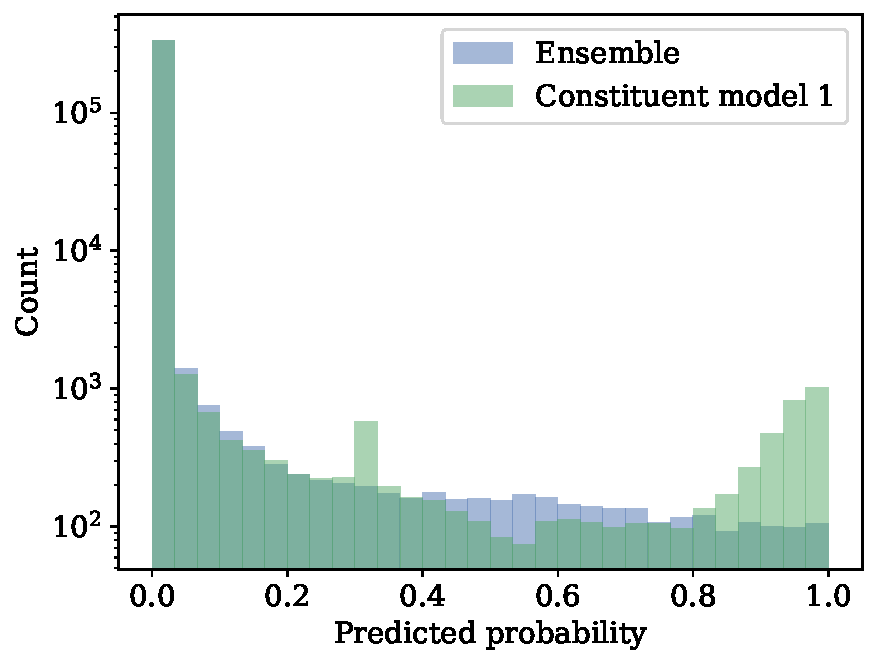
\includegraphics[width=1\columnwidth]{python_plotting/histogram_ensemble_and_single_model.pdf}
        % \caption{}
        % \label{fig_discussion:histogram_ensemble_and_single_model}
    \end{subfigure}
    \caption[Calibration curve for the uncalibrated stroke recognition model and empirical distribution of predicted probabilities.]{Calibration curve for the uncalibrated ensemble model with median F1-score also reported in \cref{tab_retrospective:table3-occlusion-analysis, fig_retrospective:figure1-roc-curve} (left) and the histogram of predicted probabilities (right).}
\end{figure}

% \subsectionP{Ensembling technique}
% To form an ensemble from several models, we need a method to form a single prediction from the outputs of the individual models.
% To allow us to evaluate an impact score for each word feature in our ablation study, we wanted our ensemble to provide not only predictions but also associated probability scores on a continuous scale. A majority voting scheme would only provide as many different scores as models, in our case five, which is arguably too coarse a resolution. 






\lesstodo[inline]{Discuss the calibration of the stroke model and report calibration curve.}
\lesstodo[inline]{Report the results of calibrating the stroke model using e.g. Platt scaling or Isotonic scaling.} % https://scikit-learn.org/stable/modules/calibration.html


% \lesstodo[inline]{Maybe mention MultiQT paper \parencite{havtorn_multiqt_2020}.}
